

\part{Prologue}


\section{External Architecture}

\autoref{fig:external_architecture} illustrates the \giraf[] launcher component. The component provides one service and have one dependency. The services it provides is based on demands from the surrounding components of the \giraf[] platform, which can be seen in \autoref{cmn:fig:architecture}. The illustrated service provides a way for launched \girafapp[]s to determine which guardian launched the application in question, and with which child profile. The illustrated dependency represents the need for being able to read and update profile data. The service which fulfill this dependency is provided by Oasis. 

As seen on \autoref{cmn:fig:architecture}, Oasis is available for the launcher to use. This database stores the modulated data, including the guardian and child profiles.


\begin{figure}[h]
	\centering
	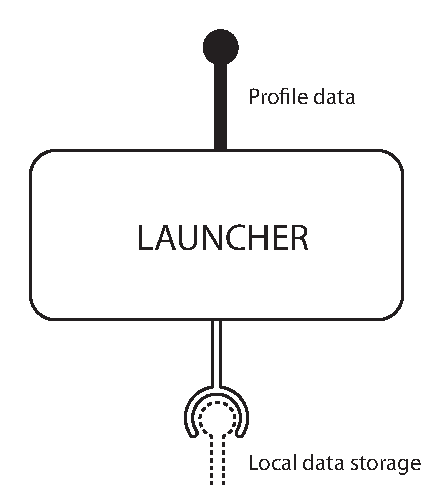
\includegraphics[width=0.5\textwidth]{gfx/external_launcher_architecture.pdf}
	\caption{The external architecture of the \giraf[] launcher.}
	\label{fig:external_architecture}
\end{figure}

%%%%%%%%%%%%%%%%%%%%%%%%%%%%%%%%%%%%%%%%%%%%%%%%%%%%%%%%%%%%%%%%%%%%%%%%%%%%%%%%%%%% COMMENT
\begin{comment}
Two external architectures are described in this section, namely those of the \giraf[] launcher, and the \guicomponents[] library.

\subsection{\giraf[] Launcher}
\label{sec:launcher_architecture}
The external architecture of the launcher can be seen in \autoref{fig:external_architecture}.
\begin{figure}[h]
	\centering
	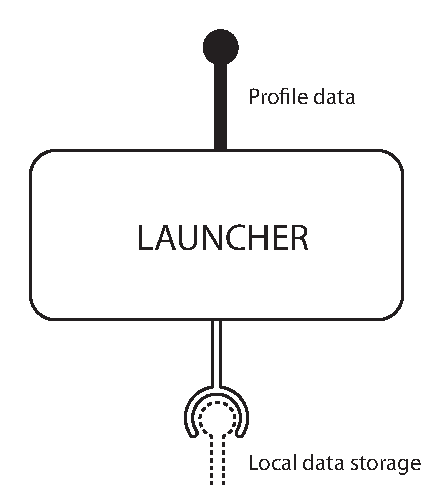
\includegraphics[width=0.5\textwidth]{gfx/external_launcher_architecture.pdf}
	\caption{The external architecture of the \giraf[] launcher.}
	\label{fig:external_architecture}
\end{figure}
The launcher provides two essential services: The ability for users to run, i.e. \textit{launch}, apps, and the provisioning of profile data to these apps. 
The launcher currently allows only \giraf[] apps to be used, but this is by design, as the launcher currently does not support addition and removal of apps. 
The profile data service allows a \guardian[] profile to select a child profile to use a given app with. 
Both the ID of the \guardian[] profile and the child profile is then provided to the app, in order to make it easy for a \guardian[] to switch between different children as needed, while maintaining specific app customizations for different profiles. \newline

The \giraf[] launcher has only one dependancy in the \giraf[] system, namely the Oasis database. 
The launcher is heavily integrated with Oasis, and as such requires the Oasis database to be installed on the device to function. 
Services utilized by the launcher include profile authentication, saving and loading of settings and app integration. 

\subsection{\guicomponents[]}
The \guicomponents[] architecture is designed to be flexible. 
The flexibility is important to keep the \guicomponents[] open and changeable by anyone involved in the development of \giraf[]. 
As such, the only architectural requirement for components that are added to \guicomponents[], is that they should be based on existing Android UI components. 
The philosophy behind this architecture, is that by using existing Android UI components, with a new layout and possible added functionality, the components are already well defined and fully supported in Android. 
The example shown in \autoref{fig:gui_comp_architecture} highlights a possible way of incorporating a component, assuming the need for a customized button: \textit{GButton}. 
\begin{figure}[h]
	\centering
	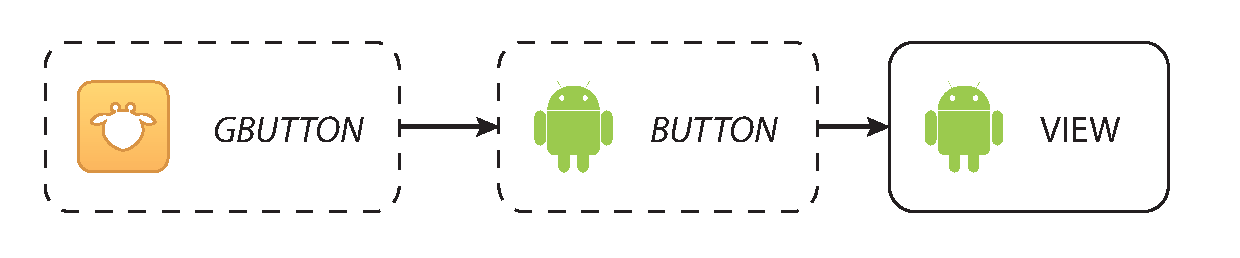
\includegraphics[width=1\textwidth]{gfx/gui_components_architecture.pdf}
	\caption{\guicomponents[] Architecture Example}
	\label{fig:gui_comp_architecture}
\end{figure}
\end{comment}
\section{Internal Architecture}

Being able to launch an \girafapp[] as a specific guardian requires that the user interacts such that the launcher knows which guardian the user represents.

Authentication is chosen, as each modulated child and guardian contains private data. QR-codes are chosen as means of authentication, as they provide a level of security.

An alternative to QR-codes could be a \emph{username-password} method, where each user have their own username, with an private password. The system is designed to have the two modes: guardian- and child mode\todo{ref til backlog}. A username-password combination requires the user to remember their credentials, whereas some \autists[] have problems with it. \todo{quote drazenko - vent paa mail fra accept}

%\myquote{Some children with autism can have a hard time remembering a username and a password}
 - Drazenko Banjak, english translation. Native language quote can be seen in \autoref{FIXME}\todo{indsaet i appendix "Nogle børn med autisme kan have svært ved at skulle huske et brugernavn og en adgangskode."}

QR codes provides a physical way of storing the user credentials and allows for other users to take responsibility of the QR-code, such as a \guardian[] carrying a QR-code of a \autist[].

QR-codes can be scanned by a built-in camera on tablets and can be printed using standard paper and printer equipment. 

QR-codes are copyable, by e.g. a copymachine, and therefore must be kept away from untrusted users, if they should not be used by people for which they were not intended.

To sum up, QR-codes are chosen because of they improve usability, despite of their ability to be copied.\todo{Ulrik, er dette i orden?}


%%%%%%%%%%%%%%%%%%%%%%%%%%%%%%%%%%%%%%%%%%%%%% COMMENT
\begin{comment}
\begin{figure}[h]
	\centering
	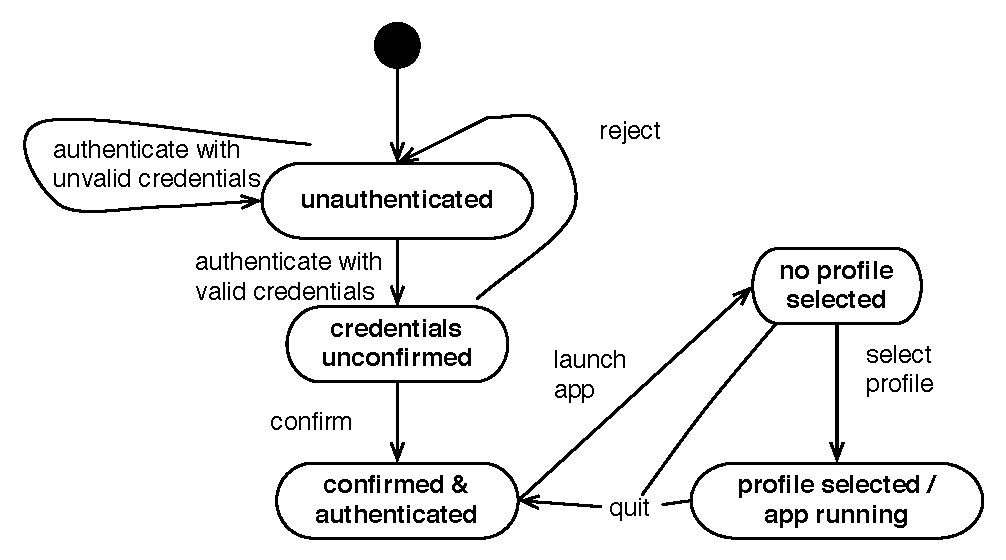
\includegraphics[width=1\textwidth]{gfx/flow-diagram2.pdf}
	\caption{Flow diagram}
	\label{fig:flow_diagram}
\end{figure}

\autoref{fig:flow_diagram} shows the state of the launcher. The first three states handles the distinction between users which are allowed to access the launchable applications, and those who are not. \todo{indsaet ref til der hvor vi fandt ud af at vi skulle have authentication}

Based on \autoref{fig:flow_diagram}, ..
\end{comment}




\section{External Architecture}

\autoref{fig:external_architecture} illustrates the \giraf[] launcher component. The component provides one service and have one dependency. The services it provides is based on demands from the surrounding components of the \giraf[] platform, which can be seen in \autoref{cmn:fig:architecture}. The illustrated service provides a way for launched \girafapp[]s to determine which guardian launched the application in question, and with which child profile. The illustrated dependency represents the need for being able to read and update profile data. The service which fulfill this dependency is provided by Oasis. 

As seen on \autoref{cmn:fig:architecture}, Oasis is available for the launcher to use. This database stores the modulated data, including the guardian and child profiles.


\begin{figure}[h]
	\centering
	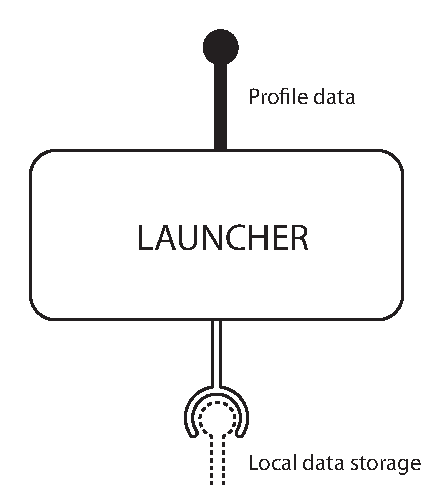
\includegraphics[width=0.5\textwidth]{gfx/external_launcher_architecture.pdf}
	\caption{The external architecture of the \giraf[] launcher.}
	\label{fig:external_architecture}
\end{figure}

%%%%%%%%%%%%%%%%%%%%%%%%%%%%%%%%%%%%%%%%%%%%%%%%%%%%%%%%%%%%%%%%%%%%%%%%%%%%%%%%%%%% COMMENT
\begin{comment}
Two external architectures are described in this section, namely those of the \giraf[] launcher, and the \guicomponents[] library.

\subsection{\giraf[] Launcher}
\label{sec:launcher_architecture}
The external architecture of the launcher can be seen in \autoref{fig:external_architecture}.
\begin{figure}[h]
	\centering
	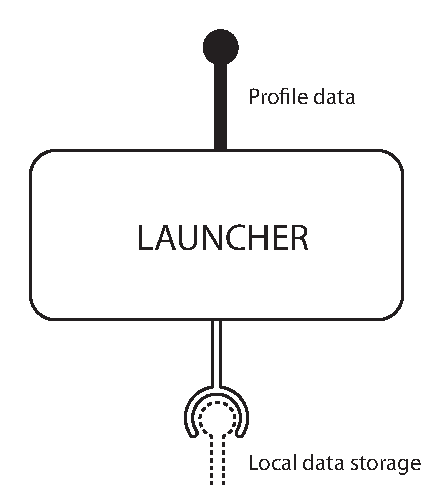
\includegraphics[width=0.5\textwidth]{gfx/external_launcher_architecture.pdf}
	\caption{The external architecture of the \giraf[] launcher.}
	\label{fig:external_architecture}
\end{figure}
The launcher provides two essential services: The ability for users to run, i.e. \textit{launch}, apps, and the provisioning of profile data to these apps. 
The launcher currently allows only \giraf[] apps to be used, but this is by design, as the launcher currently does not support addition and removal of apps. 
The profile data service allows a \guardian[] profile to select a child profile to use a given app with. 
Both the ID of the \guardian[] profile and the child profile is then provided to the app, in order to make it easy for a \guardian[] to switch between different children as needed, while maintaining specific app customizations for different profiles. \newline

The \giraf[] launcher has only one dependancy in the \giraf[] system, namely the Oasis database. 
The launcher is heavily integrated with Oasis, and as such requires the Oasis database to be installed on the device to function. 
Services utilized by the launcher include profile authentication, saving and loading of settings and app integration. 

\subsection{\guicomponents[]}
The \guicomponents[] architecture is designed to be flexible. 
The flexibility is important to keep the \guicomponents[] open and changeable by anyone involved in the development of \giraf[]. 
As such, the only architectural requirement for components that are added to \guicomponents[], is that they should be based on existing Android UI components. 
The philosophy behind this architecture, is that by using existing Android UI components, with a new layout and possible added functionality, the components are already well defined and fully supported in Android. 
The example shown in \autoref{fig:gui_comp_architecture} highlights a possible way of incorporating a component, assuming the need for a customized button: \textit{GButton}. 
\begin{figure}[h]
	\centering
	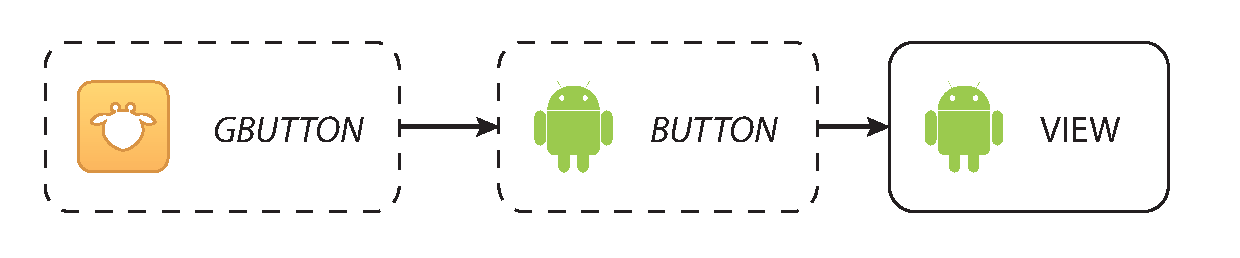
\includegraphics[width=1\textwidth]{gfx/gui_components_architecture.pdf}
	\caption{\guicomponents[] Architecture Example}
	\label{fig:gui_comp_architecture}
\end{figure}
\end{comment}
\section{Internal Architecture}

Being able to launch an \girafapp[] as a specific guardian requires that the user interacts such that the launcher knows which guardian the user represents.

Authentication is chosen, as each modulated child and guardian contains private data. QR-codes are chosen as means of authentication, as they provide a level of security.

An alternative to QR-codes could be a \emph{username-password} method, where each user have their own username, with an private password. The system is designed to have the two modes: guardian- and child mode\todo{ref til backlog}. A username-password combination requires the user to remember their credentials, whereas some \autists[] have problems with it. \todo{quote drazenko - vent paa mail fra accept}

%\myquote{Some children with autism can have a hard time remembering a username and a password}
 - Drazenko Banjak, english translation. Native language quote can be seen in \autoref{FIXME}\todo{indsaet i appendix "Nogle børn med autisme kan have svært ved at skulle huske et brugernavn og en adgangskode."}

QR codes provides a physical way of storing the user credentials and allows for other users to take responsibility of the QR-code, such as a \guardian[] carrying a QR-code of a \autist[].

QR-codes can be scanned by a built-in camera on tablets and can be printed using standard paper and printer equipment. 

QR-codes are copyable, by e.g. a copymachine, and therefore must be kept away from untrusted users, if they should not be used by people for which they were not intended.

To sum up, QR-codes are chosen because of they improve usability, despite of their ability to be copied.\todo{Ulrik, er dette i orden?}


%%%%%%%%%%%%%%%%%%%%%%%%%%%%%%%%%%%%%%%%%%%%%% COMMENT
\begin{comment}
\begin{figure}[h]
	\centering
	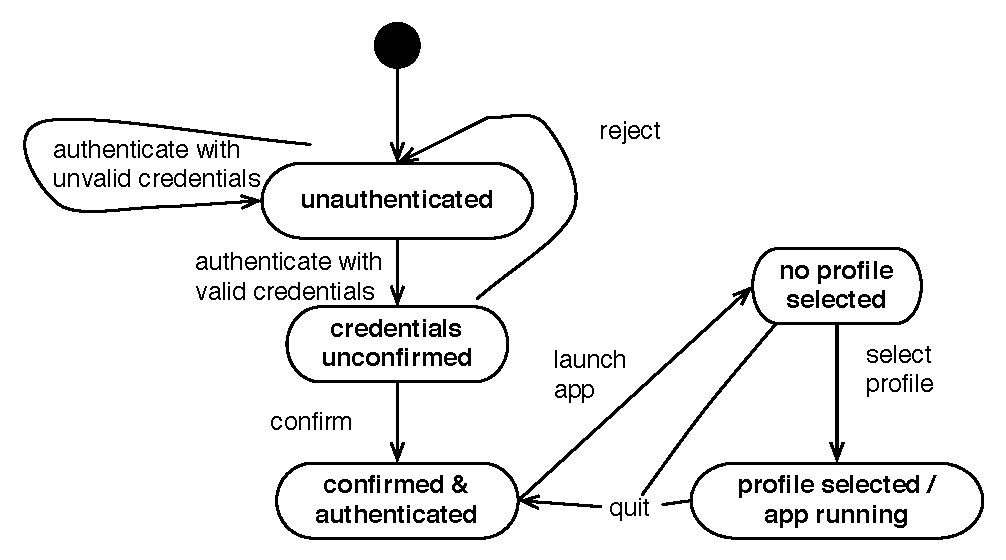
\includegraphics[width=1\textwidth]{gfx/flow-diagram2.pdf}
	\caption{Flow diagram}
	\label{fig:flow_diagram}
\end{figure}

\autoref{fig:flow_diagram} shows the state of the launcher. The first three states handles the distinction between users which are allowed to access the launchable applications, and those who are not. \todo{indsaet ref til der hvor vi fandt ud af at vi skulle have authentication}

Based on \autoref{fig:flow_diagram}, ..
\end{comment}



\cleardoublepage


\part{Process}
\chapter{Preanalysis}


\section{External Architecture}

\autoref{fig:external_architecture} illustrates the \giraf[] launcher component. The component provides one service and have one dependency. The services it provides is based on demands from the surrounding components of the \giraf[] platform, which can be seen in \autoref{cmn:fig:architecture}. The illustrated service provides a way for launched \girafapp[]s to determine which guardian launched the application in question, and with which child profile. The illustrated dependency represents the need for being able to read and update profile data. The service which fulfill this dependency is provided by Oasis. 

As seen on \autoref{cmn:fig:architecture}, Oasis is available for the launcher to use. This database stores the modulated data, including the guardian and child profiles.


\begin{figure}[h]
	\centering
	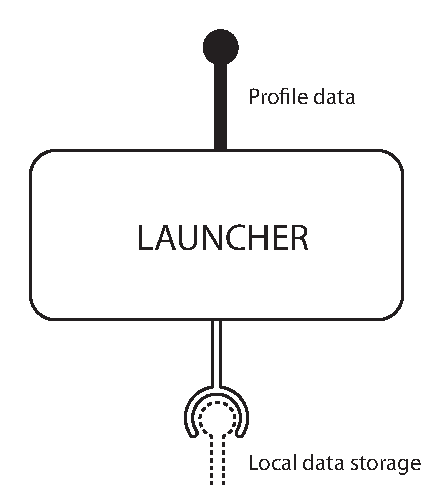
\includegraphics[width=0.5\textwidth]{gfx/external_launcher_architecture.pdf}
	\caption{The external architecture of the \giraf[] launcher.}
	\label{fig:external_architecture}
\end{figure}

%%%%%%%%%%%%%%%%%%%%%%%%%%%%%%%%%%%%%%%%%%%%%%%%%%%%%%%%%%%%%%%%%%%%%%%%%%%%%%%%%%%% COMMENT
\begin{comment}
Two external architectures are described in this section, namely those of the \giraf[] launcher, and the \guicomponents[] library.

\subsection{\giraf[] Launcher}
\label{sec:launcher_architecture}
The external architecture of the launcher can be seen in \autoref{fig:external_architecture}.
\begin{figure}[h]
	\centering
	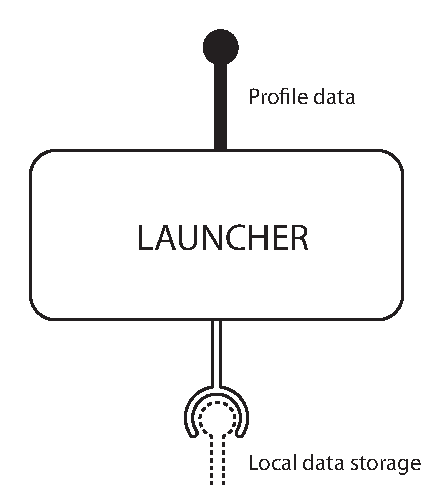
\includegraphics[width=0.5\textwidth]{gfx/external_launcher_architecture.pdf}
	\caption{The external architecture of the \giraf[] launcher.}
	\label{fig:external_architecture}
\end{figure}
The launcher provides two essential services: The ability for users to run, i.e. \textit{launch}, apps, and the provisioning of profile data to these apps. 
The launcher currently allows only \giraf[] apps to be used, but this is by design, as the launcher currently does not support addition and removal of apps. 
The profile data service allows a \guardian[] profile to select a child profile to use a given app with. 
Both the ID of the \guardian[] profile and the child profile is then provided to the app, in order to make it easy for a \guardian[] to switch between different children as needed, while maintaining specific app customizations for different profiles. \newline

The \giraf[] launcher has only one dependancy in the \giraf[] system, namely the Oasis database. 
The launcher is heavily integrated with Oasis, and as such requires the Oasis database to be installed on the device to function. 
Services utilized by the launcher include profile authentication, saving and loading of settings and app integration. 

\subsection{\guicomponents[]}
The \guicomponents[] architecture is designed to be flexible. 
The flexibility is important to keep the \guicomponents[] open and changeable by anyone involved in the development of \giraf[]. 
As such, the only architectural requirement for components that are added to \guicomponents[], is that they should be based on existing Android UI components. 
The philosophy behind this architecture, is that by using existing Android UI components, with a new layout and possible added functionality, the components are already well defined and fully supported in Android. 
The example shown in \autoref{fig:gui_comp_architecture} highlights a possible way of incorporating a component, assuming the need for a customized button: \textit{GButton}. 
\begin{figure}[h]
	\centering
	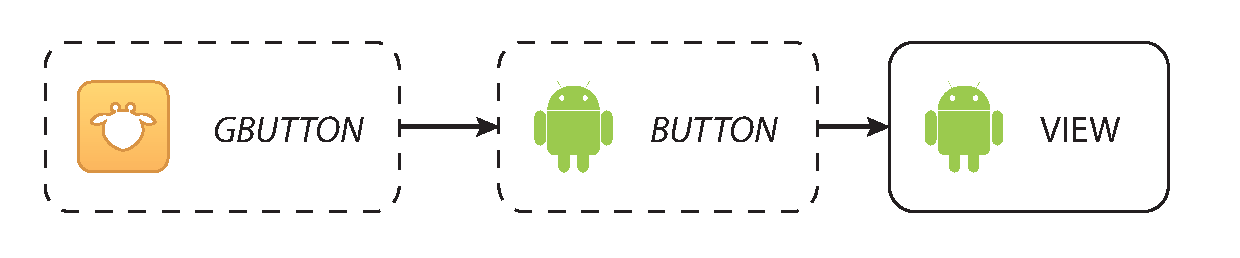
\includegraphics[width=1\textwidth]{gfx/gui_components_architecture.pdf}
	\caption{\guicomponents[] Architecture Example}
	\label{fig:gui_comp_architecture}
\end{figure}
\end{comment}
\section{Internal Architecture}

Being able to launch an \girafapp[] as a specific guardian requires that the user interacts such that the launcher knows which guardian the user represents.

Authentication is chosen, as each modulated child and guardian contains private data. QR-codes are chosen as means of authentication, as they provide a level of security.

An alternative to QR-codes could be a \emph{username-password} method, where each user have their own username, with an private password. The system is designed to have the two modes: guardian- and child mode\todo{ref til backlog}. A username-password combination requires the user to remember their credentials, whereas some \autists[] have problems with it. \todo{quote drazenko - vent paa mail fra accept}

%\myquote{Some children with autism can have a hard time remembering a username and a password}
 - Drazenko Banjak, english translation. Native language quote can be seen in \autoref{FIXME}\todo{indsaet i appendix "Nogle børn med autisme kan have svært ved at skulle huske et brugernavn og en adgangskode."}

QR codes provides a physical way of storing the user credentials and allows for other users to take responsibility of the QR-code, such as a \guardian[] carrying a QR-code of a \autist[].

QR-codes can be scanned by a built-in camera on tablets and can be printed using standard paper and printer equipment. 

QR-codes are copyable, by e.g. a copymachine, and therefore must be kept away from untrusted users, if they should not be used by people for which they were not intended.

To sum up, QR-codes are chosen because of they improve usability, despite of their ability to be copied.\todo{Ulrik, er dette i orden?}


%%%%%%%%%%%%%%%%%%%%%%%%%%%%%%%%%%%%%%%%%%%%%% COMMENT
\begin{comment}
\begin{figure}[h]
	\centering
	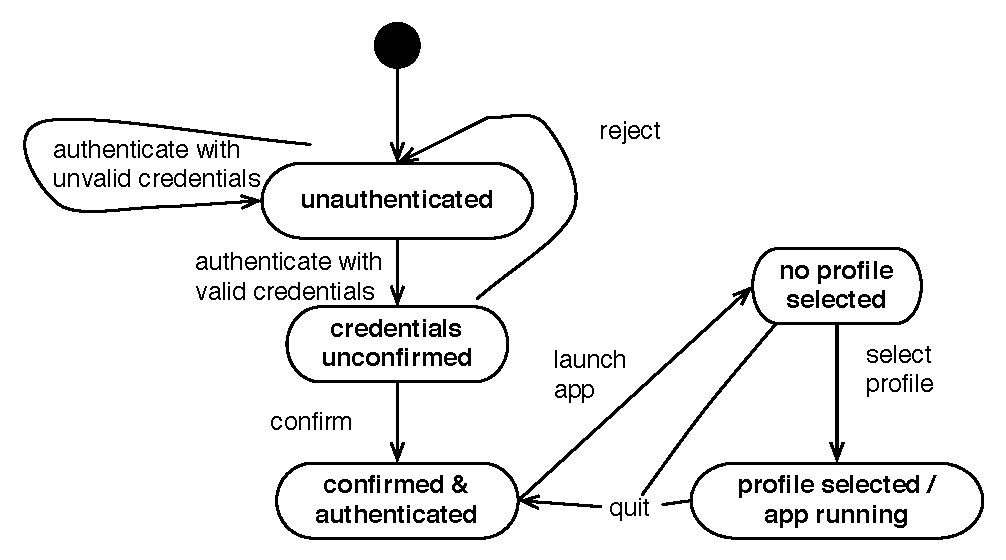
\includegraphics[width=1\textwidth]{gfx/flow-diagram2.pdf}
	\caption{Flow diagram}
	\label{fig:flow_diagram}
\end{figure}

\autoref{fig:flow_diagram} shows the state of the launcher. The first three states handles the distinction between users which are allowed to access the launchable applications, and those who are not. \todo{indsaet ref til der hvor vi fandt ud af at vi skulle have authentication}

Based on \autoref{fig:flow_diagram}, ..
\end{comment}


\chapter{Iterative Process} % Describing the process


\section{External Architecture}

\autoref{fig:external_architecture} illustrates the \giraf[] launcher component. The component provides one service and have one dependency. The services it provides is based on demands from the surrounding components of the \giraf[] platform, which can be seen in \autoref{cmn:fig:architecture}. The illustrated service provides a way for launched \girafapp[]s to determine which guardian launched the application in question, and with which child profile. The illustrated dependency represents the need for being able to read and update profile data. The service which fulfill this dependency is provided by Oasis. 

As seen on \autoref{cmn:fig:architecture}, Oasis is available for the launcher to use. This database stores the modulated data, including the guardian and child profiles.


\begin{figure}[h]
	\centering
	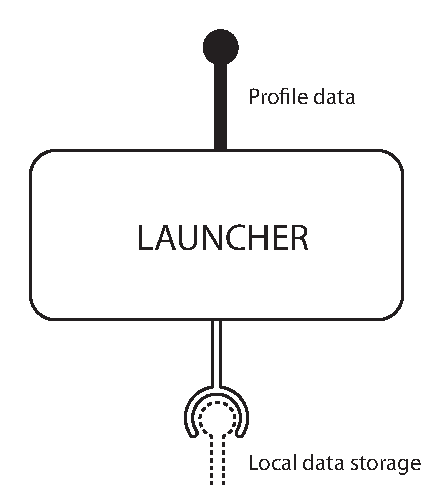
\includegraphics[width=0.5\textwidth]{gfx/external_launcher_architecture.pdf}
	\caption{The external architecture of the \giraf[] launcher.}
	\label{fig:external_architecture}
\end{figure}

%%%%%%%%%%%%%%%%%%%%%%%%%%%%%%%%%%%%%%%%%%%%%%%%%%%%%%%%%%%%%%%%%%%%%%%%%%%%%%%%%%%% COMMENT
\begin{comment}
Two external architectures are described in this section, namely those of the \giraf[] launcher, and the \guicomponents[] library.

\subsection{\giraf[] Launcher}
\label{sec:launcher_architecture}
The external architecture of the launcher can be seen in \autoref{fig:external_architecture}.
\begin{figure}[h]
	\centering
	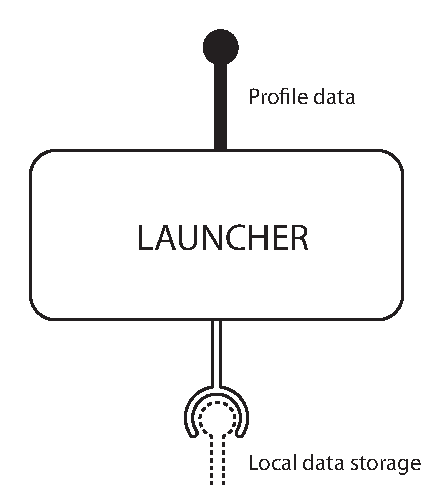
\includegraphics[width=0.5\textwidth]{gfx/external_launcher_architecture.pdf}
	\caption{The external architecture of the \giraf[] launcher.}
	\label{fig:external_architecture}
\end{figure}
The launcher provides two essential services: The ability for users to run, i.e. \textit{launch}, apps, and the provisioning of profile data to these apps. 
The launcher currently allows only \giraf[] apps to be used, but this is by design, as the launcher currently does not support addition and removal of apps. 
The profile data service allows a \guardian[] profile to select a child profile to use a given app with. 
Both the ID of the \guardian[] profile and the child profile is then provided to the app, in order to make it easy for a \guardian[] to switch between different children as needed, while maintaining specific app customizations for different profiles. \newline

The \giraf[] launcher has only one dependancy in the \giraf[] system, namely the Oasis database. 
The launcher is heavily integrated with Oasis, and as such requires the Oasis database to be installed on the device to function. 
Services utilized by the launcher include profile authentication, saving and loading of settings and app integration. 

\subsection{\guicomponents[]}
The \guicomponents[] architecture is designed to be flexible. 
The flexibility is important to keep the \guicomponents[] open and changeable by anyone involved in the development of \giraf[]. 
As such, the only architectural requirement for components that are added to \guicomponents[], is that they should be based on existing Android UI components. 
The philosophy behind this architecture, is that by using existing Android UI components, with a new layout and possible added functionality, the components are already well defined and fully supported in Android. 
The example shown in \autoref{fig:gui_comp_architecture} highlights a possible way of incorporating a component, assuming the need for a customized button: \textit{GButton}. 
\begin{figure}[h]
	\centering
	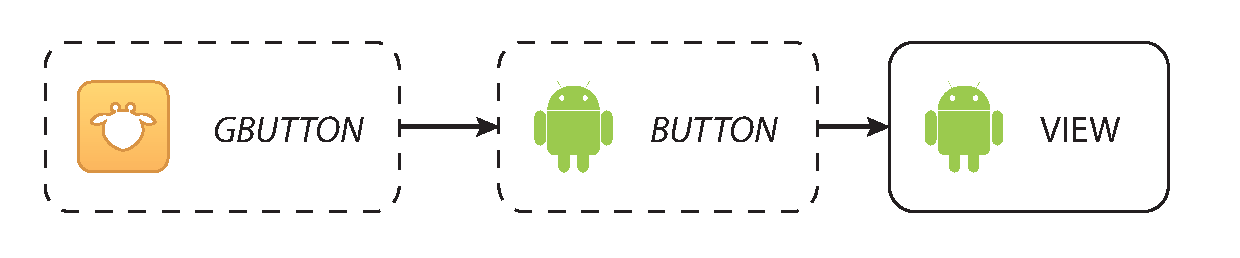
\includegraphics[width=1\textwidth]{gfx/gui_components_architecture.pdf}
	\caption{\guicomponents[] Architecture Example}
	\label{fig:gui_comp_architecture}
\end{figure}
\end{comment}
\section{Internal Architecture}

Being able to launch an \girafapp[] as a specific guardian requires that the user interacts such that the launcher knows which guardian the user represents.

Authentication is chosen, as each modulated child and guardian contains private data. QR-codes are chosen as means of authentication, as they provide a level of security.

An alternative to QR-codes could be a \emph{username-password} method, where each user have their own username, with an private password. The system is designed to have the two modes: guardian- and child mode\todo{ref til backlog}. A username-password combination requires the user to remember their credentials, whereas some \autists[] have problems with it. \todo{quote drazenko - vent paa mail fra accept}

%\myquote{Some children with autism can have a hard time remembering a username and a password}
 - Drazenko Banjak, english translation. Native language quote can be seen in \autoref{FIXME}\todo{indsaet i appendix "Nogle børn med autisme kan have svært ved at skulle huske et brugernavn og en adgangskode."}

QR codes provides a physical way of storing the user credentials and allows for other users to take responsibility of the QR-code, such as a \guardian[] carrying a QR-code of a \autist[].

QR-codes can be scanned by a built-in camera on tablets and can be printed using standard paper and printer equipment. 

QR-codes are copyable, by e.g. a copymachine, and therefore must be kept away from untrusted users, if they should not be used by people for which they were not intended.

To sum up, QR-codes are chosen because of they improve usability, despite of their ability to be copied.\todo{Ulrik, er dette i orden?}


%%%%%%%%%%%%%%%%%%%%%%%%%%%%%%%%%%%%%%%%%%%%%% COMMENT
\begin{comment}
\begin{figure}[h]
	\centering
	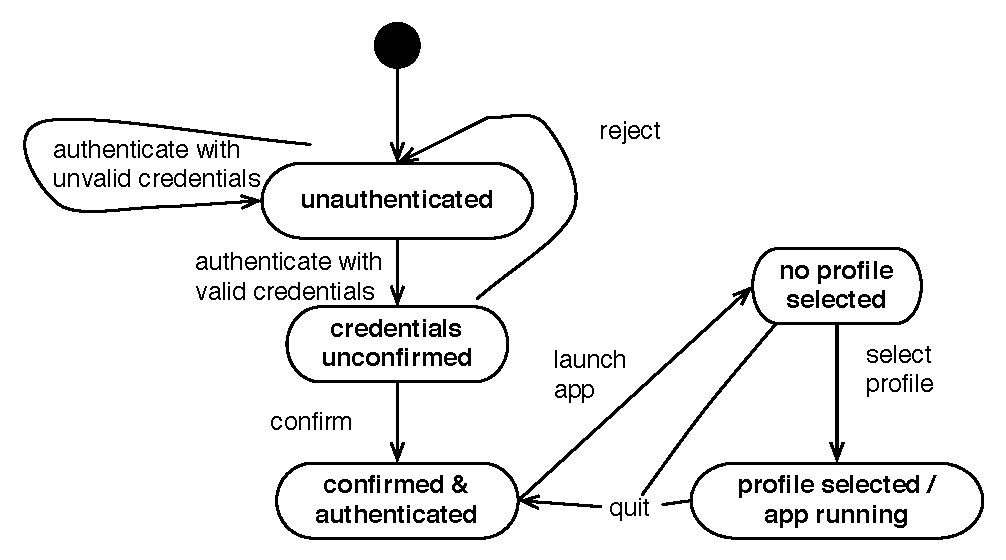
\includegraphics[width=1\textwidth]{gfx/flow-diagram2.pdf}
	\caption{Flow diagram}
	\label{fig:flow_diagram}
\end{figure}

\autoref{fig:flow_diagram} shows the state of the launcher. The first three states handles the distinction between users which are allowed to access the launchable applications, and those who are not. \todo{indsaet ref til der hvor vi fandt ud af at vi skulle have authentication}

Based on \autoref{fig:flow_diagram}, ..
\end{comment}




\section{External Architecture}

\autoref{fig:external_architecture} illustrates the \giraf[] launcher component. The component provides one service and have one dependency. The services it provides is based on demands from the surrounding components of the \giraf[] platform, which can be seen in \autoref{cmn:fig:architecture}. The illustrated service provides a way for launched \girafapp[]s to determine which guardian launched the application in question, and with which child profile. The illustrated dependency represents the need for being able to read and update profile data. The service which fulfill this dependency is provided by Oasis. 

As seen on \autoref{cmn:fig:architecture}, Oasis is available for the launcher to use. This database stores the modulated data, including the guardian and child profiles.


\begin{figure}[h]
	\centering
	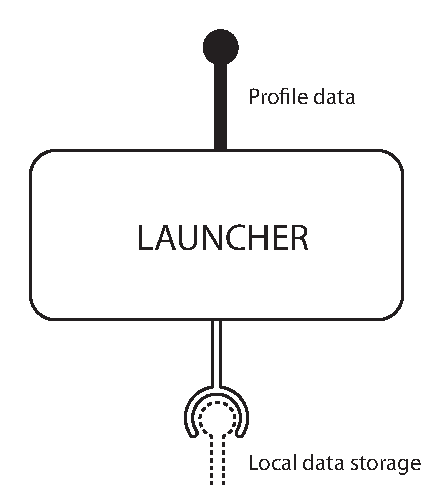
\includegraphics[width=0.5\textwidth]{gfx/external_launcher_architecture.pdf}
	\caption{The external architecture of the \giraf[] launcher.}
	\label{fig:external_architecture}
\end{figure}

%%%%%%%%%%%%%%%%%%%%%%%%%%%%%%%%%%%%%%%%%%%%%%%%%%%%%%%%%%%%%%%%%%%%%%%%%%%%%%%%%%%% COMMENT
\begin{comment}
Two external architectures are described in this section, namely those of the \giraf[] launcher, and the \guicomponents[] library.

\subsection{\giraf[] Launcher}
\label{sec:launcher_architecture}
The external architecture of the launcher can be seen in \autoref{fig:external_architecture}.
\begin{figure}[h]
	\centering
	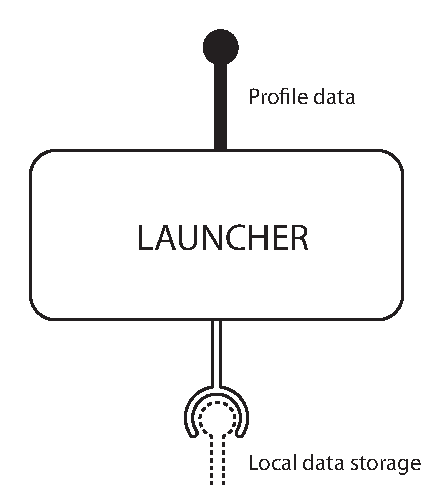
\includegraphics[width=0.5\textwidth]{gfx/external_launcher_architecture.pdf}
	\caption{The external architecture of the \giraf[] launcher.}
	\label{fig:external_architecture}
\end{figure}
The launcher provides two essential services: The ability for users to run, i.e. \textit{launch}, apps, and the provisioning of profile data to these apps. 
The launcher currently allows only \giraf[] apps to be used, but this is by design, as the launcher currently does not support addition and removal of apps. 
The profile data service allows a \guardian[] profile to select a child profile to use a given app with. 
Both the ID of the \guardian[] profile and the child profile is then provided to the app, in order to make it easy for a \guardian[] to switch between different children as needed, while maintaining specific app customizations for different profiles. \newline

The \giraf[] launcher has only one dependancy in the \giraf[] system, namely the Oasis database. 
The launcher is heavily integrated with Oasis, and as such requires the Oasis database to be installed on the device to function. 
Services utilized by the launcher include profile authentication, saving and loading of settings and app integration. 

\subsection{\guicomponents[]}
The \guicomponents[] architecture is designed to be flexible. 
The flexibility is important to keep the \guicomponents[] open and changeable by anyone involved in the development of \giraf[]. 
As such, the only architectural requirement for components that are added to \guicomponents[], is that they should be based on existing Android UI components. 
The philosophy behind this architecture, is that by using existing Android UI components, with a new layout and possible added functionality, the components are already well defined and fully supported in Android. 
The example shown in \autoref{fig:gui_comp_architecture} highlights a possible way of incorporating a component, assuming the need for a customized button: \textit{GButton}. 
\begin{figure}[h]
	\centering
	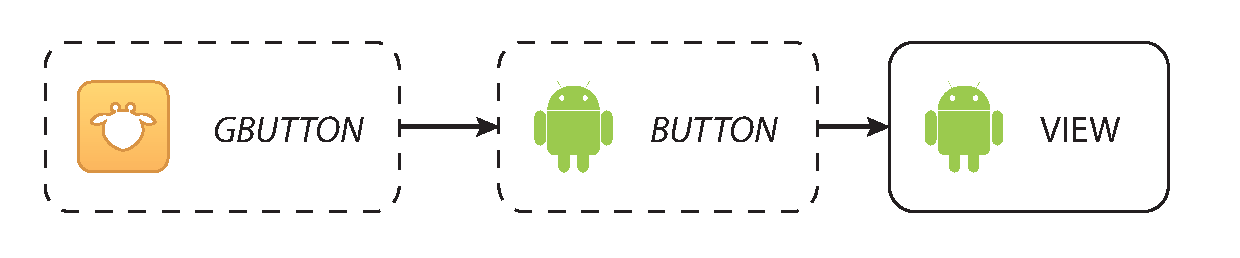
\includegraphics[width=1\textwidth]{gfx/gui_components_architecture.pdf}
	\caption{\guicomponents[] Architecture Example}
	\label{fig:gui_comp_architecture}
\end{figure}
\end{comment}
\section{Internal Architecture}

Being able to launch an \girafapp[] as a specific guardian requires that the user interacts such that the launcher knows which guardian the user represents.

Authentication is chosen, as each modulated child and guardian contains private data. QR-codes are chosen as means of authentication, as they provide a level of security.

An alternative to QR-codes could be a \emph{username-password} method, where each user have their own username, with an private password. The system is designed to have the two modes: guardian- and child mode\todo{ref til backlog}. A username-password combination requires the user to remember their credentials, whereas some \autists[] have problems with it. \todo{quote drazenko - vent paa mail fra accept}

%\myquote{Some children with autism can have a hard time remembering a username and a password}
 - Drazenko Banjak, english translation. Native language quote can be seen in \autoref{FIXME}\todo{indsaet i appendix "Nogle børn med autisme kan have svært ved at skulle huske et brugernavn og en adgangskode."}

QR codes provides a physical way of storing the user credentials and allows for other users to take responsibility of the QR-code, such as a \guardian[] carrying a QR-code of a \autist[].

QR-codes can be scanned by a built-in camera on tablets and can be printed using standard paper and printer equipment. 

QR-codes are copyable, by e.g. a copymachine, and therefore must be kept away from untrusted users, if they should not be used by people for which they were not intended.

To sum up, QR-codes are chosen because of they improve usability, despite of their ability to be copied.\todo{Ulrik, er dette i orden?}


%%%%%%%%%%%%%%%%%%%%%%%%%%%%%%%%%%%%%%%%%%%%%% COMMENT
\begin{comment}
\begin{figure}[h]
	\centering
	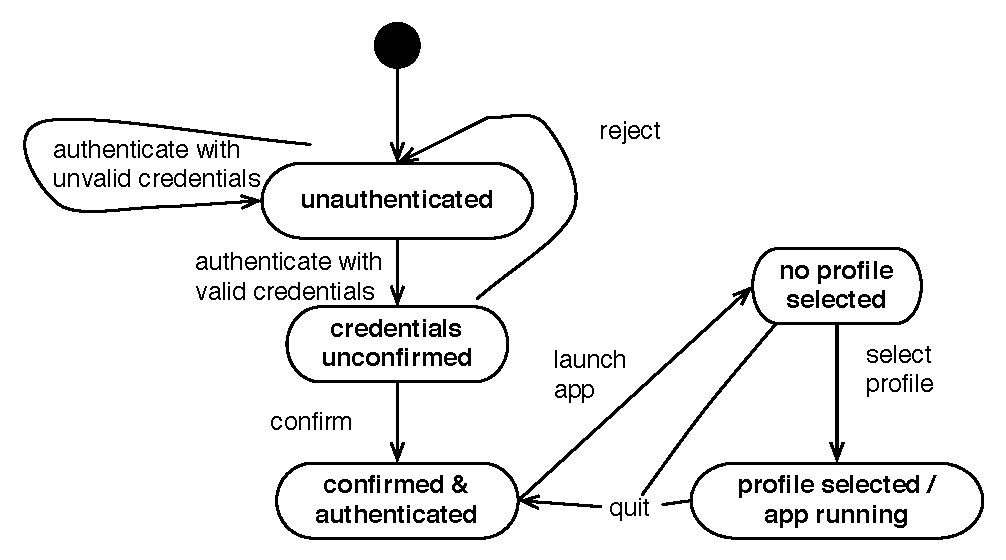
\includegraphics[width=1\textwidth]{gfx/flow-diagram2.pdf}
	\caption{Flow diagram}
	\label{fig:flow_diagram}
\end{figure}

\autoref{fig:flow_diagram} shows the state of the launcher. The first three states handles the distinction between users which are allowed to access the launchable applications, and those who are not. \todo{indsaet ref til der hvor vi fandt ud af at vi skulle have authentication}

Based on \autoref{fig:flow_diagram}, ..
\end{comment}




%\ctparttext{The \emph{product} part explains the state of the product as of our delivery of this report without any of the features of the backlog which have not been marked as done.\todo{tjek om dette holder naar backloggen er skrevet}}
%\part{Product}
\ctparttext{The \emph{design} part explains all the product specific decisions as of our delivery of this report without any of the features of the backlog which are not marked as done.

\todo{tjek om dette holder naar backloggen er skrevet}}
\part{Design}

\chapter{Design}


\section{External Architecture}

\autoref{fig:external_architecture} illustrates the \giraf[] launcher component. The component provides one service and have one dependency. The services it provides is based on demands from the surrounding components of the \giraf[] platform, which can be seen in \autoref{cmn:fig:architecture}. The illustrated service provides a way for launched \girafapp[]s to determine which guardian launched the application in question, and with which child profile. The illustrated dependency represents the need for being able to read and update profile data. The service which fulfill this dependency is provided by Oasis. 

As seen on \autoref{cmn:fig:architecture}, Oasis is available for the launcher to use. This database stores the modulated data, including the guardian and child profiles.


\begin{figure}[h]
	\centering
	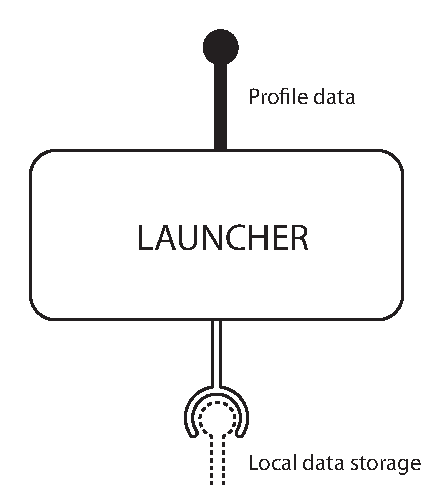
\includegraphics[width=0.5\textwidth]{gfx/external_launcher_architecture.pdf}
	\caption{The external architecture of the \giraf[] launcher.}
	\label{fig:external_architecture}
\end{figure}

%%%%%%%%%%%%%%%%%%%%%%%%%%%%%%%%%%%%%%%%%%%%%%%%%%%%%%%%%%%%%%%%%%%%%%%%%%%%%%%%%%%% COMMENT
\begin{comment}
Two external architectures are described in this section, namely those of the \giraf[] launcher, and the \guicomponents[] library.

\subsection{\giraf[] Launcher}
\label{sec:launcher_architecture}
The external architecture of the launcher can be seen in \autoref{fig:external_architecture}.
\begin{figure}[h]
	\centering
	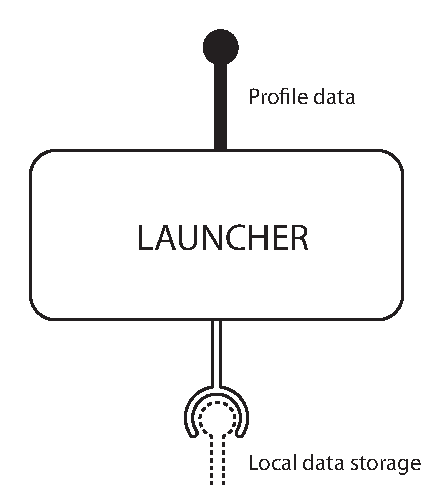
\includegraphics[width=0.5\textwidth]{gfx/external_launcher_architecture.pdf}
	\caption{The external architecture of the \giraf[] launcher.}
	\label{fig:external_architecture}
\end{figure}
The launcher provides two essential services: The ability for users to run, i.e. \textit{launch}, apps, and the provisioning of profile data to these apps. 
The launcher currently allows only \giraf[] apps to be used, but this is by design, as the launcher currently does not support addition and removal of apps. 
The profile data service allows a \guardian[] profile to select a child profile to use a given app with. 
Both the ID of the \guardian[] profile and the child profile is then provided to the app, in order to make it easy for a \guardian[] to switch between different children as needed, while maintaining specific app customizations for different profiles. \newline

The \giraf[] launcher has only one dependancy in the \giraf[] system, namely the Oasis database. 
The launcher is heavily integrated with Oasis, and as such requires the Oasis database to be installed on the device to function. 
Services utilized by the launcher include profile authentication, saving and loading of settings and app integration. 

\subsection{\guicomponents[]}
The \guicomponents[] architecture is designed to be flexible. 
The flexibility is important to keep the \guicomponents[] open and changeable by anyone involved in the development of \giraf[]. 
As such, the only architectural requirement for components that are added to \guicomponents[], is that they should be based on existing Android UI components. 
The philosophy behind this architecture, is that by using existing Android UI components, with a new layout and possible added functionality, the components are already well defined and fully supported in Android. 
The example shown in \autoref{fig:gui_comp_architecture} highlights a possible way of incorporating a component, assuming the need for a customized button: \textit{GButton}. 
\begin{figure}[h]
	\centering
	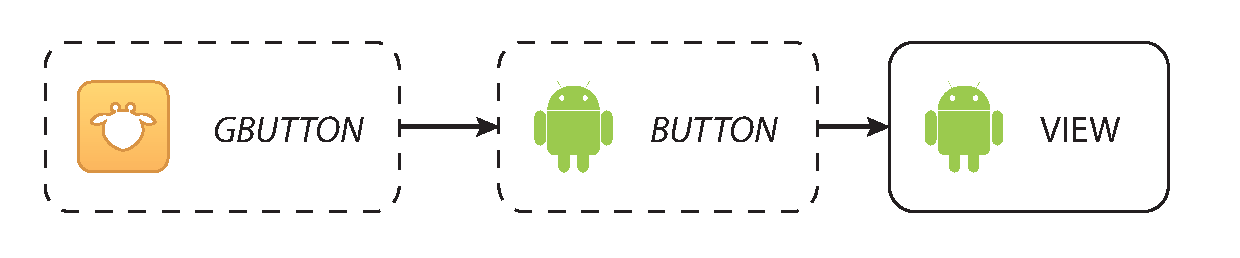
\includegraphics[width=1\textwidth]{gfx/gui_components_architecture.pdf}
	\caption{\guicomponents[] Architecture Example}
	\label{fig:gui_comp_architecture}
\end{figure}
\end{comment}
\section{Internal Architecture}

Being able to launch an \girafapp[] as a specific guardian requires that the user interacts such that the launcher knows which guardian the user represents.

Authentication is chosen, as each modulated child and guardian contains private data. QR-codes are chosen as means of authentication, as they provide a level of security.

An alternative to QR-codes could be a \emph{username-password} method, where each user have their own username, with an private password. The system is designed to have the two modes: guardian- and child mode\todo{ref til backlog}. A username-password combination requires the user to remember their credentials, whereas some \autists[] have problems with it. \todo{quote drazenko - vent paa mail fra accept}

%\myquote{Some children with autism can have a hard time remembering a username and a password}
 - Drazenko Banjak, english translation. Native language quote can be seen in \autoref{FIXME}\todo{indsaet i appendix "Nogle børn med autisme kan have svært ved at skulle huske et brugernavn og en adgangskode."}

QR codes provides a physical way of storing the user credentials and allows for other users to take responsibility of the QR-code, such as a \guardian[] carrying a QR-code of a \autist[].

QR-codes can be scanned by a built-in camera on tablets and can be printed using standard paper and printer equipment. 

QR-codes are copyable, by e.g. a copymachine, and therefore must be kept away from untrusted users, if they should not be used by people for which they were not intended.

To sum up, QR-codes are chosen because of they improve usability, despite of their ability to be copied.\todo{Ulrik, er dette i orden?}


%%%%%%%%%%%%%%%%%%%%%%%%%%%%%%%%%%%%%%%%%%%%%% COMMENT
\begin{comment}
\begin{figure}[h]
	\centering
	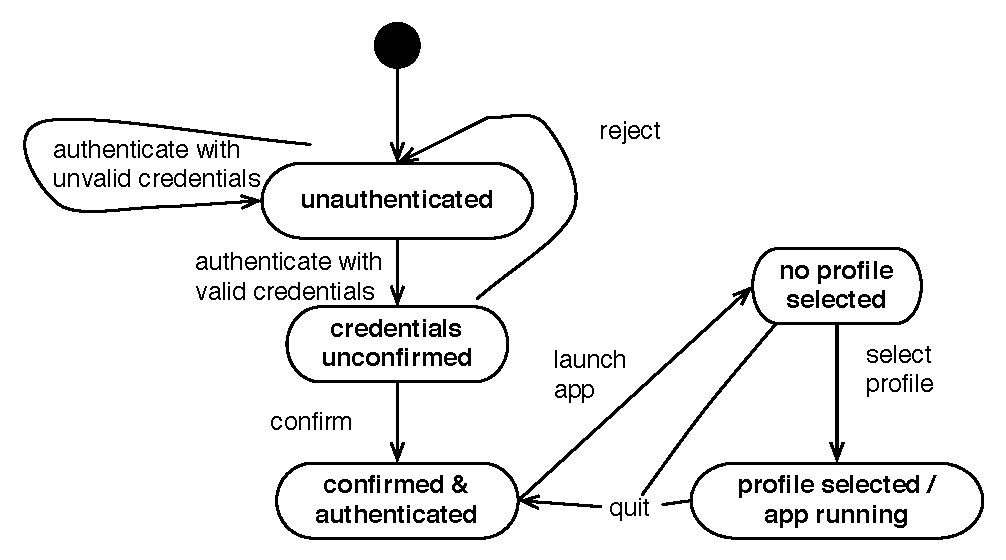
\includegraphics[width=1\textwidth]{gfx/flow-diagram2.pdf}
	\caption{Flow diagram}
	\label{fig:flow_diagram}
\end{figure}

\autoref{fig:flow_diagram} shows the state of the launcher. The first three states handles the distinction between users which are allowed to access the launchable applications, and those who are not. \todo{indsaet ref til der hvor vi fandt ud af at vi skulle have authentication}

Based on \autoref{fig:flow_diagram}, ..
\end{comment}


\chapter{Implementation}


\section{External Architecture}

\autoref{fig:external_architecture} illustrates the \giraf[] launcher component. The component provides one service and have one dependency. The services it provides is based on demands from the surrounding components of the \giraf[] platform, which can be seen in \autoref{cmn:fig:architecture}. The illustrated service provides a way for launched \girafapp[]s to determine which guardian launched the application in question, and with which child profile. The illustrated dependency represents the need for being able to read and update profile data. The service which fulfill this dependency is provided by Oasis. 

As seen on \autoref{cmn:fig:architecture}, Oasis is available for the launcher to use. This database stores the modulated data, including the guardian and child profiles.


\begin{figure}[h]
	\centering
	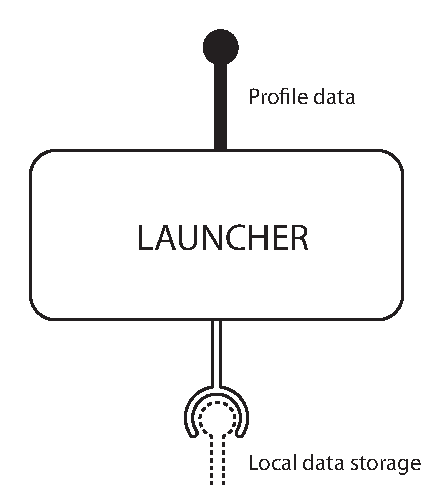
\includegraphics[width=0.5\textwidth]{gfx/external_launcher_architecture.pdf}
	\caption{The external architecture of the \giraf[] launcher.}
	\label{fig:external_architecture}
\end{figure}

%%%%%%%%%%%%%%%%%%%%%%%%%%%%%%%%%%%%%%%%%%%%%%%%%%%%%%%%%%%%%%%%%%%%%%%%%%%%%%%%%%%% COMMENT
\begin{comment}
Two external architectures are described in this section, namely those of the \giraf[] launcher, and the \guicomponents[] library.

\subsection{\giraf[] Launcher}
\label{sec:launcher_architecture}
The external architecture of the launcher can be seen in \autoref{fig:external_architecture}.
\begin{figure}[h]
	\centering
	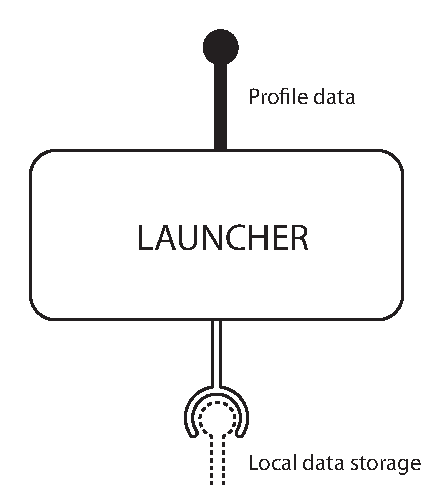
\includegraphics[width=0.5\textwidth]{gfx/external_launcher_architecture.pdf}
	\caption{The external architecture of the \giraf[] launcher.}
	\label{fig:external_architecture}
\end{figure}
The launcher provides two essential services: The ability for users to run, i.e. \textit{launch}, apps, and the provisioning of profile data to these apps. 
The launcher currently allows only \giraf[] apps to be used, but this is by design, as the launcher currently does not support addition and removal of apps. 
The profile data service allows a \guardian[] profile to select a child profile to use a given app with. 
Both the ID of the \guardian[] profile and the child profile is then provided to the app, in order to make it easy for a \guardian[] to switch between different children as needed, while maintaining specific app customizations for different profiles. \newline

The \giraf[] launcher has only one dependancy in the \giraf[] system, namely the Oasis database. 
The launcher is heavily integrated with Oasis, and as such requires the Oasis database to be installed on the device to function. 
Services utilized by the launcher include profile authentication, saving and loading of settings and app integration. 

\subsection{\guicomponents[]}
The \guicomponents[] architecture is designed to be flexible. 
The flexibility is important to keep the \guicomponents[] open and changeable by anyone involved in the development of \giraf[]. 
As such, the only architectural requirement for components that are added to \guicomponents[], is that they should be based on existing Android UI components. 
The philosophy behind this architecture, is that by using existing Android UI components, with a new layout and possible added functionality, the components are already well defined and fully supported in Android. 
The example shown in \autoref{fig:gui_comp_architecture} highlights a possible way of incorporating a component, assuming the need for a customized button: \textit{GButton}. 
\begin{figure}[h]
	\centering
	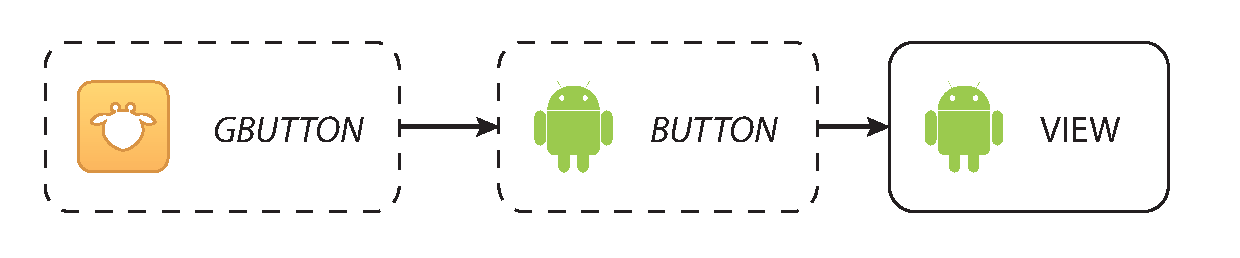
\includegraphics[width=1\textwidth]{gfx/gui_components_architecture.pdf}
	\caption{\guicomponents[] Architecture Example}
	\label{fig:gui_comp_architecture}
\end{figure}
\end{comment}
\section{Internal Architecture}

Being able to launch an \girafapp[] as a specific guardian requires that the user interacts such that the launcher knows which guardian the user represents.

Authentication is chosen, as each modulated child and guardian contains private data. QR-codes are chosen as means of authentication, as they provide a level of security.

An alternative to QR-codes could be a \emph{username-password} method, where each user have their own username, with an private password. The system is designed to have the two modes: guardian- and child mode\todo{ref til backlog}. A username-password combination requires the user to remember their credentials, whereas some \autists[] have problems with it. \todo{quote drazenko - vent paa mail fra accept}

%\myquote{Some children with autism can have a hard time remembering a username and a password}
 - Drazenko Banjak, english translation. Native language quote can be seen in \autoref{FIXME}\todo{indsaet i appendix "Nogle børn med autisme kan have svært ved at skulle huske et brugernavn og en adgangskode."}

QR codes provides a physical way of storing the user credentials and allows for other users to take responsibility of the QR-code, such as a \guardian[] carrying a QR-code of a \autist[].

QR-codes can be scanned by a built-in camera on tablets and can be printed using standard paper and printer equipment. 

QR-codes are copyable, by e.g. a copymachine, and therefore must be kept away from untrusted users, if they should not be used by people for which they were not intended.

To sum up, QR-codes are chosen because of they improve usability, despite of their ability to be copied.\todo{Ulrik, er dette i orden?}


%%%%%%%%%%%%%%%%%%%%%%%%%%%%%%%%%%%%%%%%%%%%%% COMMENT
\begin{comment}
\begin{figure}[h]
	\centering
	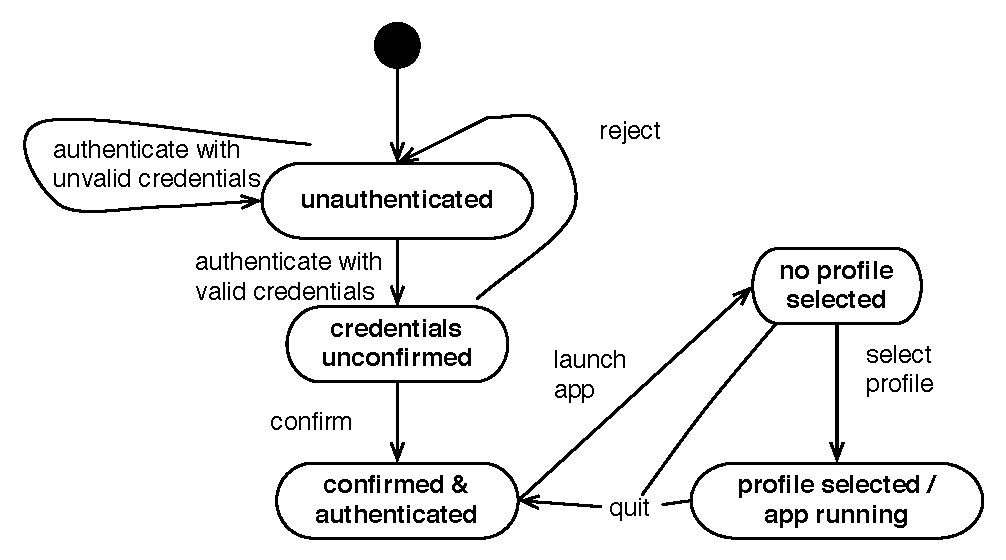
\includegraphics[width=1\textwidth]{gfx/flow-diagram2.pdf}
	\caption{Flow diagram}
	\label{fig:flow_diagram}
\end{figure}

\autoref{fig:flow_diagram} shows the state of the launcher. The first three states handles the distinction between users which are allowed to access the launchable applications, and those who are not. \todo{indsaet ref til der hvor vi fandt ud af at vi skulle have authentication}

Based on \autoref{fig:flow_diagram}, ..
\end{comment}


\chapter{Test and Verification}


\section{External Architecture}

\autoref{fig:external_architecture} illustrates the \giraf[] launcher component. The component provides one service and have one dependency. The services it provides is based on demands from the surrounding components of the \giraf[] platform, which can be seen in \autoref{cmn:fig:architecture}. The illustrated service provides a way for launched \girafapp[]s to determine which guardian launched the application in question, and with which child profile. The illustrated dependency represents the need for being able to read and update profile data. The service which fulfill this dependency is provided by Oasis. 

As seen on \autoref{cmn:fig:architecture}, Oasis is available for the launcher to use. This database stores the modulated data, including the guardian and child profiles.


\begin{figure}[h]
	\centering
	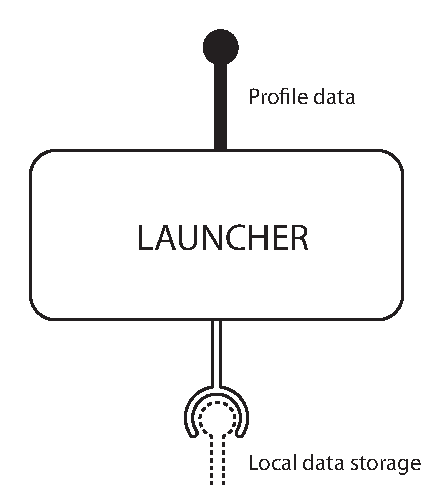
\includegraphics[width=0.5\textwidth]{gfx/external_launcher_architecture.pdf}
	\caption{The external architecture of the \giraf[] launcher.}
	\label{fig:external_architecture}
\end{figure}

%%%%%%%%%%%%%%%%%%%%%%%%%%%%%%%%%%%%%%%%%%%%%%%%%%%%%%%%%%%%%%%%%%%%%%%%%%%%%%%%%%%% COMMENT
\begin{comment}
Two external architectures are described in this section, namely those of the \giraf[] launcher, and the \guicomponents[] library.

\subsection{\giraf[] Launcher}
\label{sec:launcher_architecture}
The external architecture of the launcher can be seen in \autoref{fig:external_architecture}.
\begin{figure}[h]
	\centering
	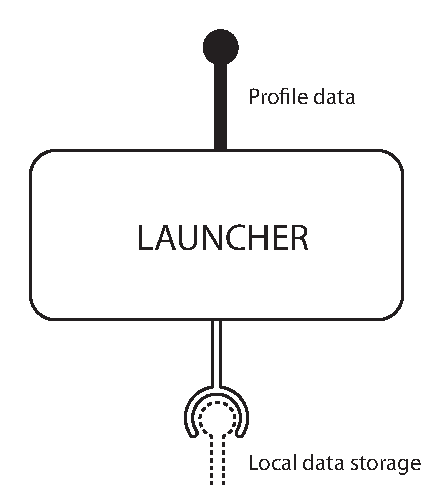
\includegraphics[width=0.5\textwidth]{gfx/external_launcher_architecture.pdf}
	\caption{The external architecture of the \giraf[] launcher.}
	\label{fig:external_architecture}
\end{figure}
The launcher provides two essential services: The ability for users to run, i.e. \textit{launch}, apps, and the provisioning of profile data to these apps. 
The launcher currently allows only \giraf[] apps to be used, but this is by design, as the launcher currently does not support addition and removal of apps. 
The profile data service allows a \guardian[] profile to select a child profile to use a given app with. 
Both the ID of the \guardian[] profile and the child profile is then provided to the app, in order to make it easy for a \guardian[] to switch between different children as needed, while maintaining specific app customizations for different profiles. \newline

The \giraf[] launcher has only one dependancy in the \giraf[] system, namely the Oasis database. 
The launcher is heavily integrated with Oasis, and as such requires the Oasis database to be installed on the device to function. 
Services utilized by the launcher include profile authentication, saving and loading of settings and app integration. 

\subsection{\guicomponents[]}
The \guicomponents[] architecture is designed to be flexible. 
The flexibility is important to keep the \guicomponents[] open and changeable by anyone involved in the development of \giraf[]. 
As such, the only architectural requirement for components that are added to \guicomponents[], is that they should be based on existing Android UI components. 
The philosophy behind this architecture, is that by using existing Android UI components, with a new layout and possible added functionality, the components are already well defined and fully supported in Android. 
The example shown in \autoref{fig:gui_comp_architecture} highlights a possible way of incorporating a component, assuming the need for a customized button: \textit{GButton}. 
\begin{figure}[h]
	\centering
	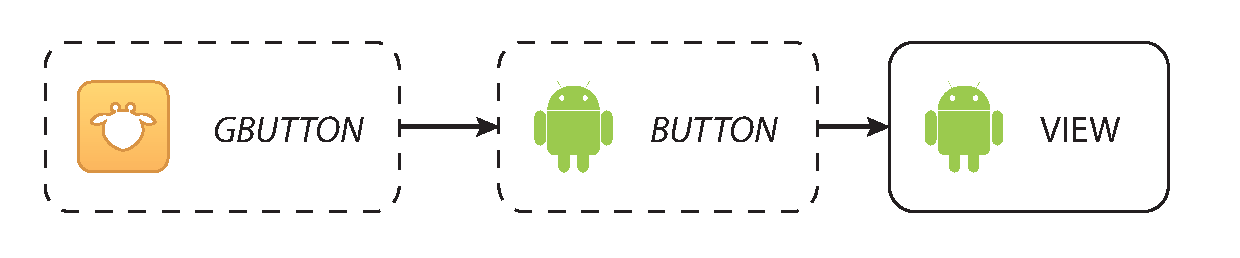
\includegraphics[width=1\textwidth]{gfx/gui_components_architecture.pdf}
	\caption{\guicomponents[] Architecture Example}
	\label{fig:gui_comp_architecture}
\end{figure}
\end{comment}
\section{Internal Architecture}

Being able to launch an \girafapp[] as a specific guardian requires that the user interacts such that the launcher knows which guardian the user represents.

Authentication is chosen, as each modulated child and guardian contains private data. QR-codes are chosen as means of authentication, as they provide a level of security.

An alternative to QR-codes could be a \emph{username-password} method, where each user have their own username, with an private password. The system is designed to have the two modes: guardian- and child mode\todo{ref til backlog}. A username-password combination requires the user to remember their credentials, whereas some \autists[] have problems with it. \todo{quote drazenko - vent paa mail fra accept}

%\myquote{Some children with autism can have a hard time remembering a username and a password}
 - Drazenko Banjak, english translation. Native language quote can be seen in \autoref{FIXME}\todo{indsaet i appendix "Nogle børn med autisme kan have svært ved at skulle huske et brugernavn og en adgangskode."}

QR codes provides a physical way of storing the user credentials and allows for other users to take responsibility of the QR-code, such as a \guardian[] carrying a QR-code of a \autist[].

QR-codes can be scanned by a built-in camera on tablets and can be printed using standard paper and printer equipment. 

QR-codes are copyable, by e.g. a copymachine, and therefore must be kept away from untrusted users, if they should not be used by people for which they were not intended.

To sum up, QR-codes are chosen because of they improve usability, despite of their ability to be copied.\todo{Ulrik, er dette i orden?}


%%%%%%%%%%%%%%%%%%%%%%%%%%%%%%%%%%%%%%%%%%%%%% COMMENT
\begin{comment}
\begin{figure}[h]
	\centering
	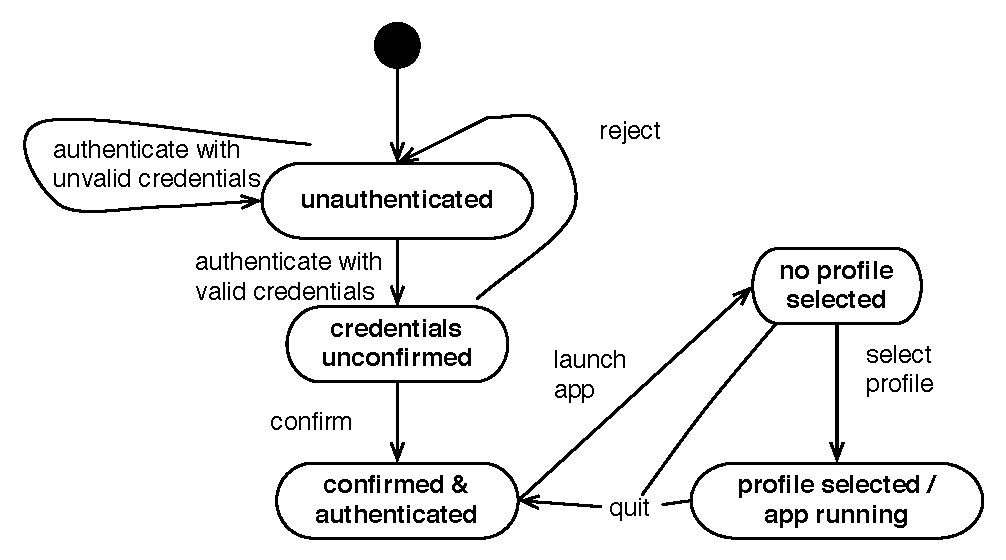
\includegraphics[width=1\textwidth]{gfx/flow-diagram2.pdf}
	\caption{Flow diagram}
	\label{fig:flow_diagram}
\end{figure}

\autoref{fig:flow_diagram} shows the state of the launcher. The first three states handles the distinction between users which are allowed to access the launchable applications, and those who are not. \todo{indsaet ref til der hvor vi fandt ud af at vi skulle have authentication}

Based on \autoref{fig:flow_diagram}, ..
\end{comment}





\part{Epilogue}


\section{External Architecture}

\autoref{fig:external_architecture} illustrates the \giraf[] launcher component. The component provides one service and have one dependency. The services it provides is based on demands from the surrounding components of the \giraf[] platform, which can be seen in \autoref{cmn:fig:architecture}. The illustrated service provides a way for launched \girafapp[]s to determine which guardian launched the application in question, and with which child profile. The illustrated dependency represents the need for being able to read and update profile data. The service which fulfill this dependency is provided by Oasis. 

As seen on \autoref{cmn:fig:architecture}, Oasis is available for the launcher to use. This database stores the modulated data, including the guardian and child profiles.


\begin{figure}[h]
	\centering
	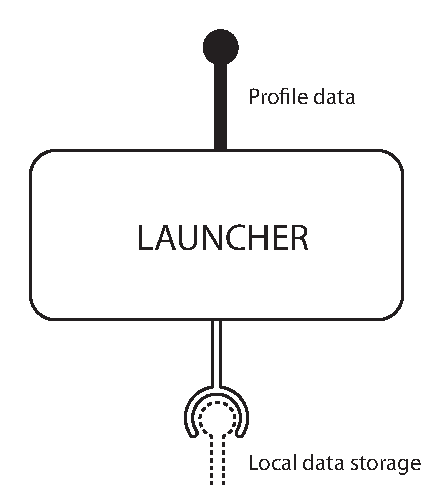
\includegraphics[width=0.5\textwidth]{gfx/external_launcher_architecture.pdf}
	\caption{The external architecture of the \giraf[] launcher.}
	\label{fig:external_architecture}
\end{figure}

%%%%%%%%%%%%%%%%%%%%%%%%%%%%%%%%%%%%%%%%%%%%%%%%%%%%%%%%%%%%%%%%%%%%%%%%%%%%%%%%%%%% COMMENT
\begin{comment}
Two external architectures are described in this section, namely those of the \giraf[] launcher, and the \guicomponents[] library.

\subsection{\giraf[] Launcher}
\label{sec:launcher_architecture}
The external architecture of the launcher can be seen in \autoref{fig:external_architecture}.
\begin{figure}[h]
	\centering
	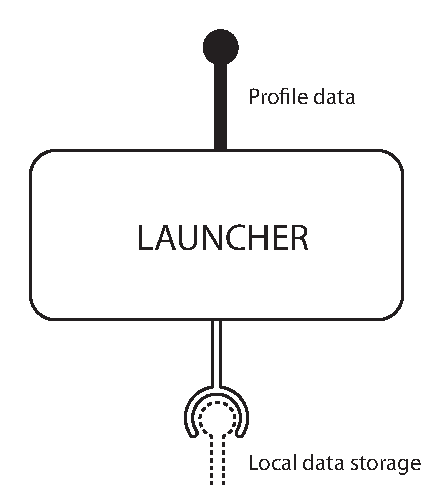
\includegraphics[width=0.5\textwidth]{gfx/external_launcher_architecture.pdf}
	\caption{The external architecture of the \giraf[] launcher.}
	\label{fig:external_architecture}
\end{figure}
The launcher provides two essential services: The ability for users to run, i.e. \textit{launch}, apps, and the provisioning of profile data to these apps. 
The launcher currently allows only \giraf[] apps to be used, but this is by design, as the launcher currently does not support addition and removal of apps. 
The profile data service allows a \guardian[] profile to select a child profile to use a given app with. 
Both the ID of the \guardian[] profile and the child profile is then provided to the app, in order to make it easy for a \guardian[] to switch between different children as needed, while maintaining specific app customizations for different profiles. \newline

The \giraf[] launcher has only one dependancy in the \giraf[] system, namely the Oasis database. 
The launcher is heavily integrated with Oasis, and as such requires the Oasis database to be installed on the device to function. 
Services utilized by the launcher include profile authentication, saving and loading of settings and app integration. 

\subsection{\guicomponents[]}
The \guicomponents[] architecture is designed to be flexible. 
The flexibility is important to keep the \guicomponents[] open and changeable by anyone involved in the development of \giraf[]. 
As such, the only architectural requirement for components that are added to \guicomponents[], is that they should be based on existing Android UI components. 
The philosophy behind this architecture, is that by using existing Android UI components, with a new layout and possible added functionality, the components are already well defined and fully supported in Android. 
The example shown in \autoref{fig:gui_comp_architecture} highlights a possible way of incorporating a component, assuming the need for a customized button: \textit{GButton}. 
\begin{figure}[h]
	\centering
	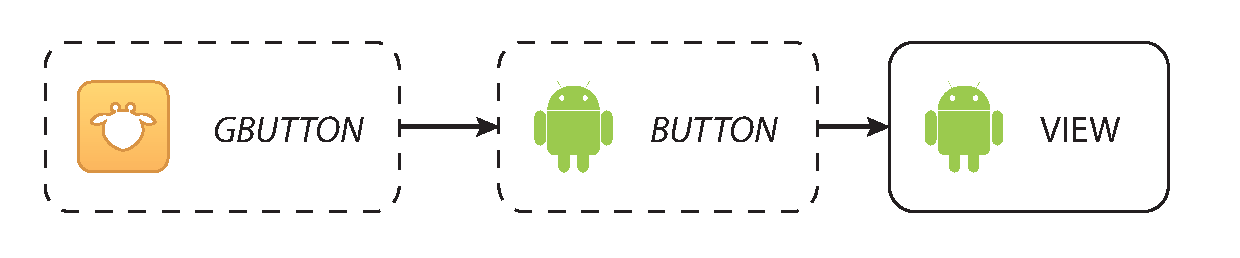
\includegraphics[width=1\textwidth]{gfx/gui_components_architecture.pdf}
	\caption{\guicomponents[] Architecture Example}
	\label{fig:gui_comp_architecture}
\end{figure}
\end{comment}
\section{Internal Architecture}

Being able to launch an \girafapp[] as a specific guardian requires that the user interacts such that the launcher knows which guardian the user represents.

Authentication is chosen, as each modulated child and guardian contains private data. QR-codes are chosen as means of authentication, as they provide a level of security.

An alternative to QR-codes could be a \emph{username-password} method, where each user have their own username, with an private password. The system is designed to have the two modes: guardian- and child mode\todo{ref til backlog}. A username-password combination requires the user to remember their credentials, whereas some \autists[] have problems with it. \todo{quote drazenko - vent paa mail fra accept}

%\myquote{Some children with autism can have a hard time remembering a username and a password}
 - Drazenko Banjak, english translation. Native language quote can be seen in \autoref{FIXME}\todo{indsaet i appendix "Nogle børn med autisme kan have svært ved at skulle huske et brugernavn og en adgangskode."}

QR codes provides a physical way of storing the user credentials and allows for other users to take responsibility of the QR-code, such as a \guardian[] carrying a QR-code of a \autist[].

QR-codes can be scanned by a built-in camera on tablets and can be printed using standard paper and printer equipment. 

QR-codes are copyable, by e.g. a copymachine, and therefore must be kept away from untrusted users, if they should not be used by people for which they were not intended.

To sum up, QR-codes are chosen because of they improve usability, despite of their ability to be copied.\todo{Ulrik, er dette i orden?}


%%%%%%%%%%%%%%%%%%%%%%%%%%%%%%%%%%%%%%%%%%%%%% COMMENT
\begin{comment}
\begin{figure}[h]
	\centering
	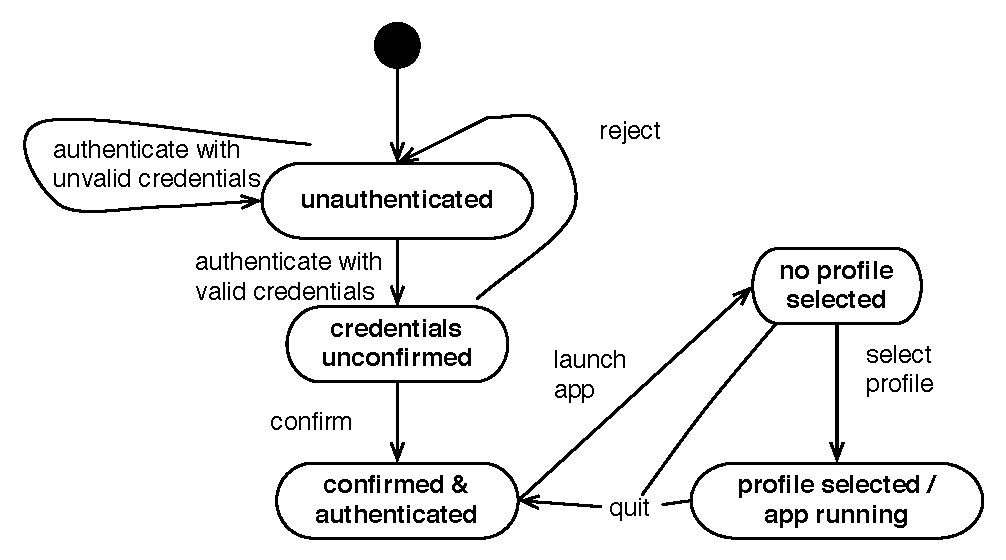
\includegraphics[width=1\textwidth]{gfx/flow-diagram2.pdf}
	\caption{Flow diagram}
	\label{fig:flow_diagram}
\end{figure}

\autoref{fig:flow_diagram} shows the state of the launcher. The first three states handles the distinction between users which are allowed to access the launchable applications, and those who are not. \todo{indsaet ref til der hvor vi fandt ud af at vi skulle have authentication}

Based on \autoref{fig:flow_diagram}, ..
\end{comment}



\part{Appendix} % The appendix
